\section{Part 2: Laplace Input Perturbation}\label{sec:p2}
\subsection{Mechanism and fixed experimental protocol}
For a raw normalized image $X$, the assignment prescribes independent noise at each pixel:
\begin{equation}
 X'=X+\xi,\qquad \xi_{ij}\overset{\mathrm{iid}}{\sim}\operatorname{Laplace}(0,b),
 \qquad p(\xi\mid b)=\frac{1}{2b}\exp\left(-\frac{|\xi|}{b}\right),\quad b>0.\label{eq:laplace}
\end{equation}
Because the network receives $z=1-X$, raw-image addition becomes $z'=1-X'=z-\xi$. At $b=0$, the implementation returns an unchanged clone without random draws.

Each run generates one fixed perturbed copy of each client's training data and reuses it for 80 rounds. Labels remain unchanged and noisy inputs are never clipped to $[0,1]$. Scale is in normalized pixel units. Training, validation, and test evaluation all use clean inputs.

Sequential FedAvg uses $C=0.10$, $E=3$, learning rate 0.3, and batch size 32. Seven scales, $b\in\{0,0.025,0.05,0.10,0.20,0.40,0.80\}$, are evaluated at seeds 2026--2028. Initialization, participation, and minibatches are matched across scales. NumPy PCG64 generates noise on CPU from keys incorporating seed, client ID, and scale; identical values are transferred to CUDA. Because scale enters the key, different scales have separate noise realizations.

The protocol fixes round 80 for all 21 scale-comparison checkpoints and separately evaluates the validation-best $b=0.10$, seed-2026 model for Question 1. Before test scoring, the scale recommendation is fixed by a maximum two-percentage-point decrease in mean final validation accuracy relative to $b=0$.

\subsection{Question 1: the detailed perturbed-data run}
For $b=0.10$, seed 2026, validation selects round 80. Clean training/validation accuracies are 72.37\%/70.72\% and losses are 0.986190/1.119120. Test accuracy is \textbf{71.64\%} (2,594/3,621), distinct from the 70.97\% three-seed mean at this scale. \Cref{fig:dpaccuracy} shows accuracy against the matched clean run; \cref{fig:dploss} provides supporting cross-entropy curves.

\begin{figure}[htbp]
\centering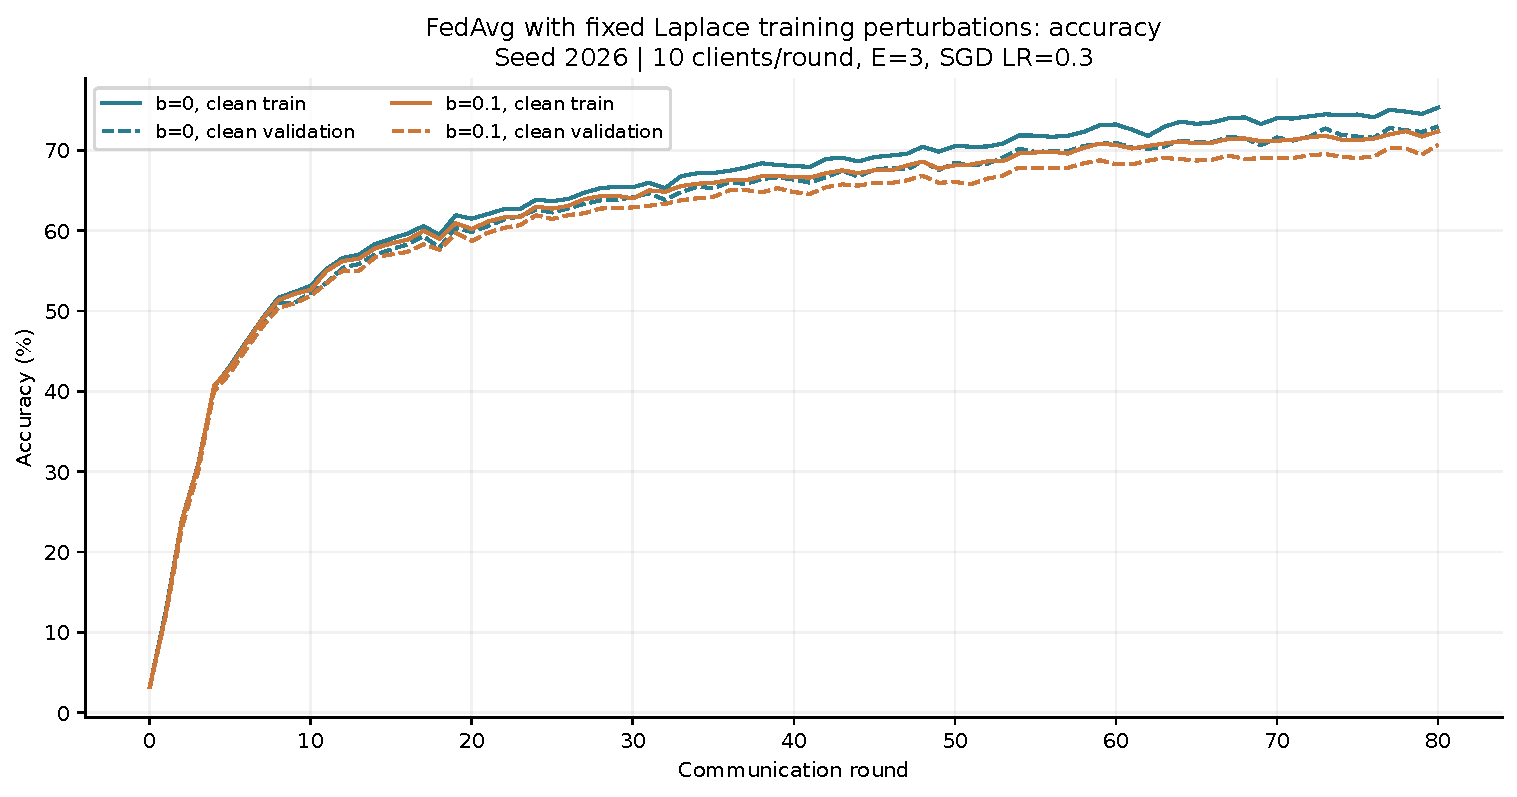
\includegraphics[width=0.9\linewidth]{figures/part2/dp_accuracy_convergence.pdf}
\caption{Part 2 Question 1: clean training and validation accuracy after training on fixed perturbed inputs, $b=0.10$ versus $b=0$, seed 2026. Both use ten clients per round and $E=3$. The noisy run's validation-best checkpoint is round 80.}\label{fig:dpaccuracy}
\end{figure}


\subsection{Questions 2--3: utility across scales and the recommendation}
\begin{table}[htbp]
\centering
\caption{Round-80 clean accuracy across seeds 2026--2028. Training values are means; validation and test show mean accuracy (\%) $\pm$ one sample SD (percentage points).}\label{tab:noisegrid}
\begin{tabular}{rrrr}
\toprule
$b$ & Training (\%) & Validation (\%) & Held-out test (\%)\\
\midrule
0 & 74.97 & $72.40\pm0.57$ & $73.38\pm0.66$\\
0.025 & 74.83 & $72.13\pm0.60$ & $73.16\pm0.65$\\
0.05 & 74.15 & $71.80\pm0.73$ & $72.66\pm0.55$\\
0.10 & 72.16 & $70.05\pm0.58$ & $70.97\pm0.57$\\
0.20 & 66.55 & $64.76\pm0.83$ & $66.06\pm0.90$\\
0.40 & 58.91 & $57.98\pm0.50$ & $58.79\pm0.54$\\
0.80 & 36.77 & $35.57\pm1.76$ & $37.15\pm1.92$\\
\bottomrule
\end{tabular}
\end{table}
\begin{figure}[htbp]
\centering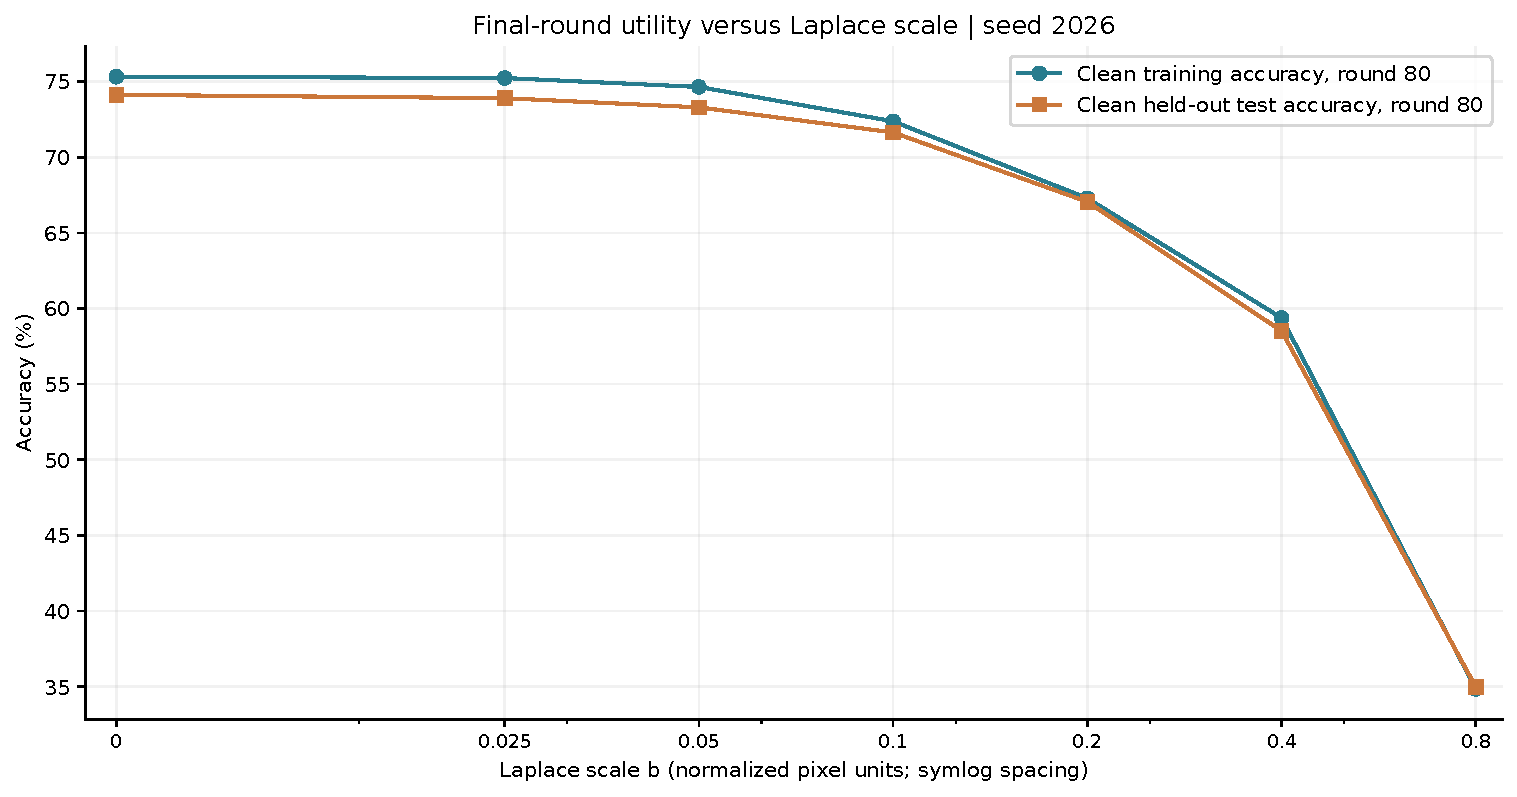
\includegraphics[width=0.9\linewidth]{figures/part2/dp_accuracy_vs_noise_scale.pdf}
\caption{Final clean training and test accuracy versus noise scale, seed 2026, round 80. The symlog axis is linear below $b=0.025$. Three-seed means appear in \cref{tab:noisegrid,fig:dpseeds}.}\label{fig:dpscale}
\end{figure}
\begin{figure}[htbp]
\centering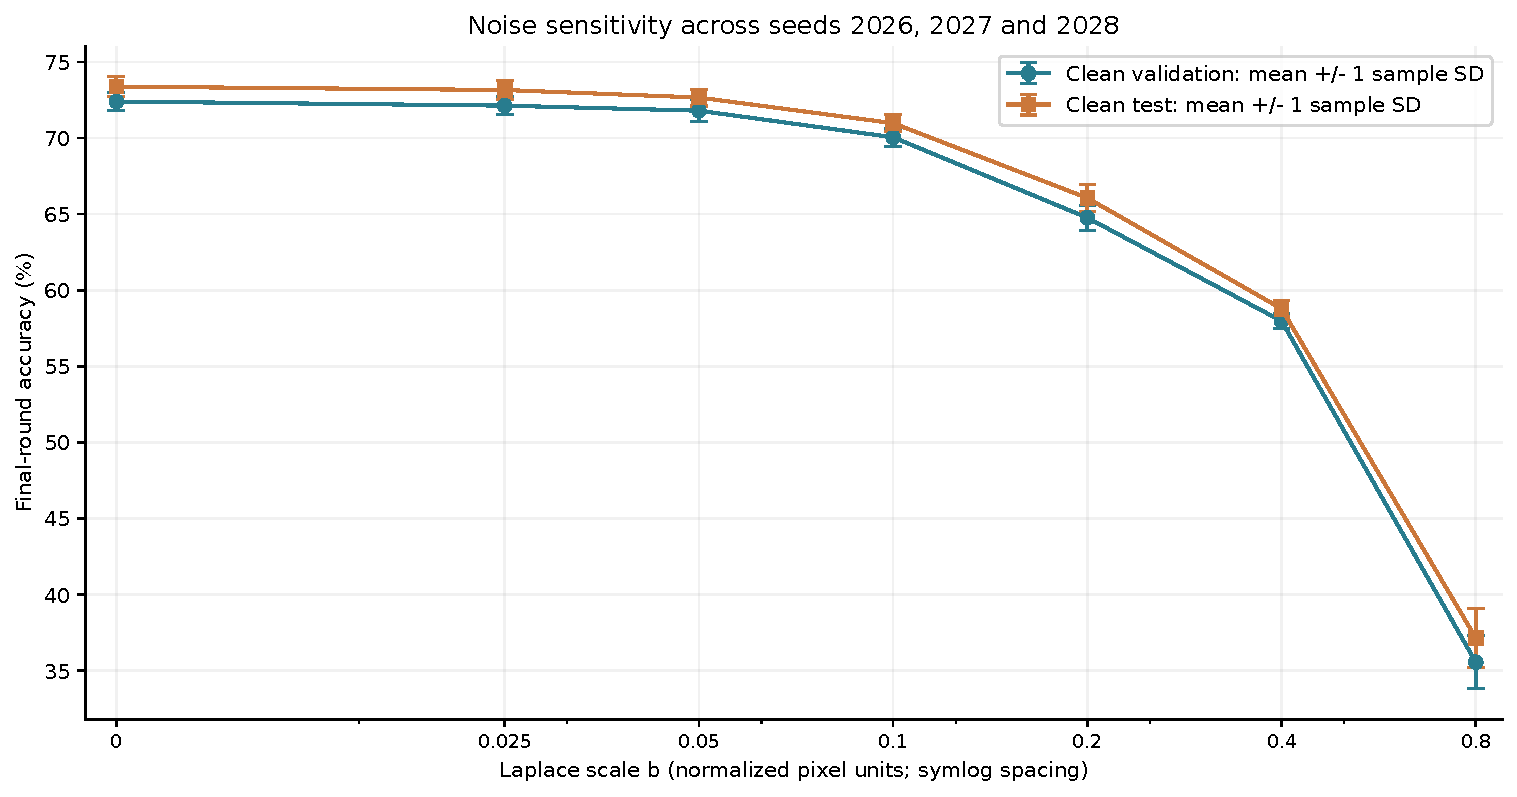
\includegraphics[width=0.9\linewidth]{figures/part2/dp_noise_seed_stability.pdf}
\caption{Mean final validation and test accuracy over three seeds, with sample-SD error bars. Every point uses round 80; no best-checkpoint results enter this plot. Larger error bars at $b=0.8$ indicate increased variation among these three training runs.}\label{fig:dpseeds}
\end{figure}

Training, validation, and test means decrease across the tested grid. Relative to the matched $b=0$ mean test accuracy of 73.38\%, $b=0.05$ loses 0.72 points and $b=0.8$ loses 36.22 points. The decline in both training and test accuracy indicates impaired signal learning under the fixed optimizer, rather than merely a wider generalization gap.

We adopted a two-percentage-point validation-accuracy tolerance as a practical utility constraint: it limits the absolute reduction in classification performance while allowing the strongest tested perturbation within that limit. This application-level choice is neither a statistical significance boundary nor a formal privacy requirement. We select the largest tested noise scale for which the mean final validation accuracy decreases by no more than two percentage points relative to the clean baseline:
\begin{equation}
\overline{A}_{\mathrm{val}}(0)-\overline{A}_{\mathrm{val}}(b)\le0.02,
\qquad A_{\mathrm{val}}\in[0,1].\label{eq:selection}
\end{equation}
The accuracy threshold is $72.39998\%-2\pp=70.39998\%$. At $b=0.05$, validation accuracy is 71.79647\%, a 0.60351-point decrease; at $b=0.10$, it is 70.04838\%, a 2.35159-point decrease. Thus \textbf{$b=0.05$ is the largest tested positive scale satisfying the criterion}, with pixel RMS distortion 0.07072 and mean test accuracy 72.65949\%. Test results describe this frozen choice and do not determine it.

Increasing $b$ from 0.10 to 0.20 reduces mean validation accuracy by a further 5.29 percentage points, from 70.05\% to 64.76\%, while mean test accuracy falls from 70.97\% to 66.06\%. Although larger $b$ tightens the hypothetical Laplace privacy bound for a fixed sensitivity, even these scales give very loose whole-image bounds (\cref{sec:privacy}). We therefore choose $b=0.05$ for the assignment's empirical distortion--utility comparison, not as a deployment recommendation for verified image-level privacy.

\subsection{Scientific Validation and Edge Cases}\label{sec:p2validation}
\subsubsection{Noise-law correctness: moments, quantiles, and tails}
Noise-law validation checks scale, shape, and tails against complementary Laplace properties:
\begin{equation}
\mathbb{E}[\xi]=0,\quad \mathbb{E}|\xi|=b,\quad
\operatorname{Var}(\xi)=2b^2,\quad
\Pr(|\xi|>3b)=e^{-3}.\label{eq:moments}
\end{equation}
At each of $b=0.025,0.10,0.80$, one million float32 draws are summarized in float64. Moments, seven quantiles between probabilities 0.01 and 0.99, and the $3b$ tail are checked against conservative six-standard-error thresholds. The mean SE is $\sqrt{2}b/\sqrt{N}$, the tail SE is $\sqrt{p(1-p)/N}$ for $p=e^{-3}$, and the variance SE is approximately $\sqrt{20}b^2/\sqrt{N}$, using fourth moment $24b^4$.

\begin{table}[htbp]
\centering
\caption{Million-sample distribution checks at each scale. The theoretical tail probability is $e^{-3}=0.0497871$ for all rows.}\label{tab:moments}
\begin{tabular}{rrrrr}
\toprule
$b$ & Empirical mean & Empirical variance & $2b^2$ & Empirical $3b$ tail\\
\midrule
0.025 & $-0.00001287$ & 0.00124851 & 0.00125000 & 0.049710\\
0.10 & $0.00001731$ & 0.01997336 & 0.02000000 & 0.049737\\
0.80 & $-0.00024118$ & 1.28365398 & 1.28000000 & 0.049780\\
\bottomrule
\end{tabular}
\end{table}

At $b=0.10$, empirical 0.01/0.99 quantiles are $-0.390109$/$0.389632$, versus theoretical $\mp0.391202$. The largest standardized quantile discrepancy is 1.578 at this scale and 2.003 across scales. All checked moment, quantile, and tail deviations are at most about 2.003 SE, within the six-SE bounds. Together, \cref{tab:moments,fig:noiselaw} discriminate incorrect scale or distribution shape more effectively than a mean-only check.

\begin{figure}[htbp]
\centering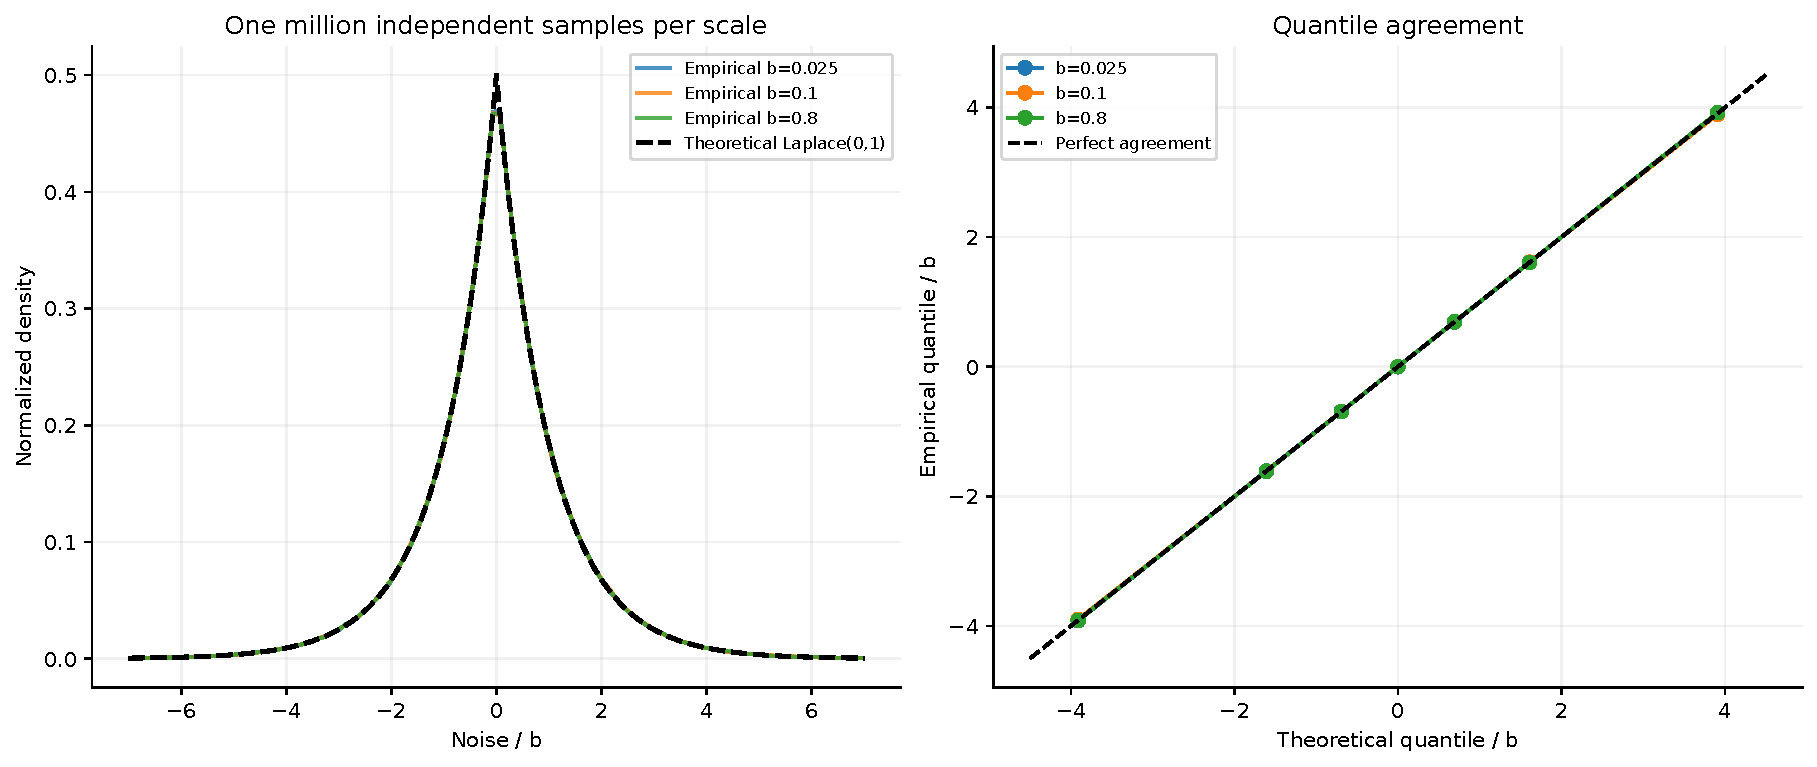
\includegraphics[width=\linewidth]{figures/part2/dp_noise_distribution_validation.pdf}
\caption{Mechanism validation: histograms of noise divided by $b$ against the unit-Laplace density, and empirical versus theoretical normalized quantiles. The three scales each use one million samples. Tail and moment checks in \cref{tab:moments} complement the plotted central density.}\label{fig:noiselaw}
\end{figure}

\subsubsection{Pixel independence, keyed reproducibility, and data isolation}
A broadcast scalar or shared-row noise bug would induce strong pixel correlations. Across 20,000 independent noise images, all 496 pairs among 32 spread pixel positions have maximum absolute correlation 0.020592, below $6/\sqrt{20{,}000}=0.042426$; mean correlation is $-0.000168$. This diagnostic detects no material linear dependence at the tested positions, while the sampling implementation supplies the IID construction.

Identical keys reproduce noise exactly; changed seeds or client IDs change it. CPU noise and its CUDA copy differ by 0.0, validating transfer rather than native-device PRNG equivalence. Two independent five-round runs at fixed $b=0.10$ also reproduce parameters and history metrics exactly.

Hash checks across all 100 clients confirm unchanged clean inputs, labels, validation tensors, and client boundaries. The held-out file hash is unchanged, computed without loading its examples during validation. Together with the separate frozen test phase, these checks verify that perturbation targets local training pixels only.

\subsubsection{Zero-noise equivalence as an end-to-end control}
The zero-noise control tests whether adding perturbation and evaluation code changes the clean algorithm. A three-round comparison matches initialization, schedules, optimizer settings, and batch seeds; parameter and all four metric differences are 0.0. The full $b=0$ runs then match their Part 1.1 counterparts for each seed 2026--2028: all 81 metric rows, 800 client selections, and round-80 parameters agree exactly.

This exact baseline recovery removes changes to splits or optimization as explanations for the positive-noise utility differences.

\subsubsection{Learning controls and noise-reuse ablation}
The synthetic noise control reaches a 100\% validation ceiling at every tested scale (\cref{app:synthetic_noise}), so the 21-run Federated EMNIST comparison provides the primary evidence for performance degradation.

To test sensitivity to noise reuse, matched 40-round real-data runs compare fixed perturbations with fresh noise each local epoch at $C=0.10,E=3$, learning rate 0.3, and batch size 32.
\begin{table}[htbp]
\centering
\caption{Separate fixed-versus-resampled-noise ablation. Values are final clean validation accuracy, using one matched seed and 40 rounds. No ablation result enters the main test grid.}\label{tab:ablation}
\begin{tabular}{rrrr}
\toprule
$b$ & Fixed (\%) & Fresh per local epoch (\%) & Difference (pp)\\
\midrule
0.10 & 64.8041 & 65.8342 & 1.0301\\
0.40 & 55.0804 & 60.1530 & 5.0726\\
\bottomrule
\end{tabular}
\end{table}
Fresh noise improves final validation accuracy by 1.03 points at $b=0.10$ and 5.07 at $b=0.40$ (\cref{tab:ablation}), suggesting that repeated exposure to fixed perturbations affects optimization. This single-seed ablation is separate from the primary fixed-noise test grid.

\subsubsection{Image distortion and client-level noise sensitivity}
Expected pixel MSE is $2b^2$, giving RMS $\sqrt{2}b$. At $b=0.05$, measured MSE/RMS are 0.00500156/0.0707217, close to 0.005/0.0707107; at $b=0.8$, RMS reaches 1.13127 (\cref{fig:distortion}). Out-of-range pixels rise from 47.10\% to 63.92\% across these scales. Even mild noise often crosses zero at background pixels, explaining the first fraction. \Cref{fig:images} illustrates the resulting image distortion.



\Cref{fig:robustness} shows each client's round-80 validation change from its same-seed $b=0$ control, averaged over three seeds and ordered by training-label entropy. Losses are widespread at larger scales but uneven: client 72 loses 8.93 points at $b=0.10$, while client 27 loses 68.33 at $b=0.8$.

\begin{figure}[htbp]
\centering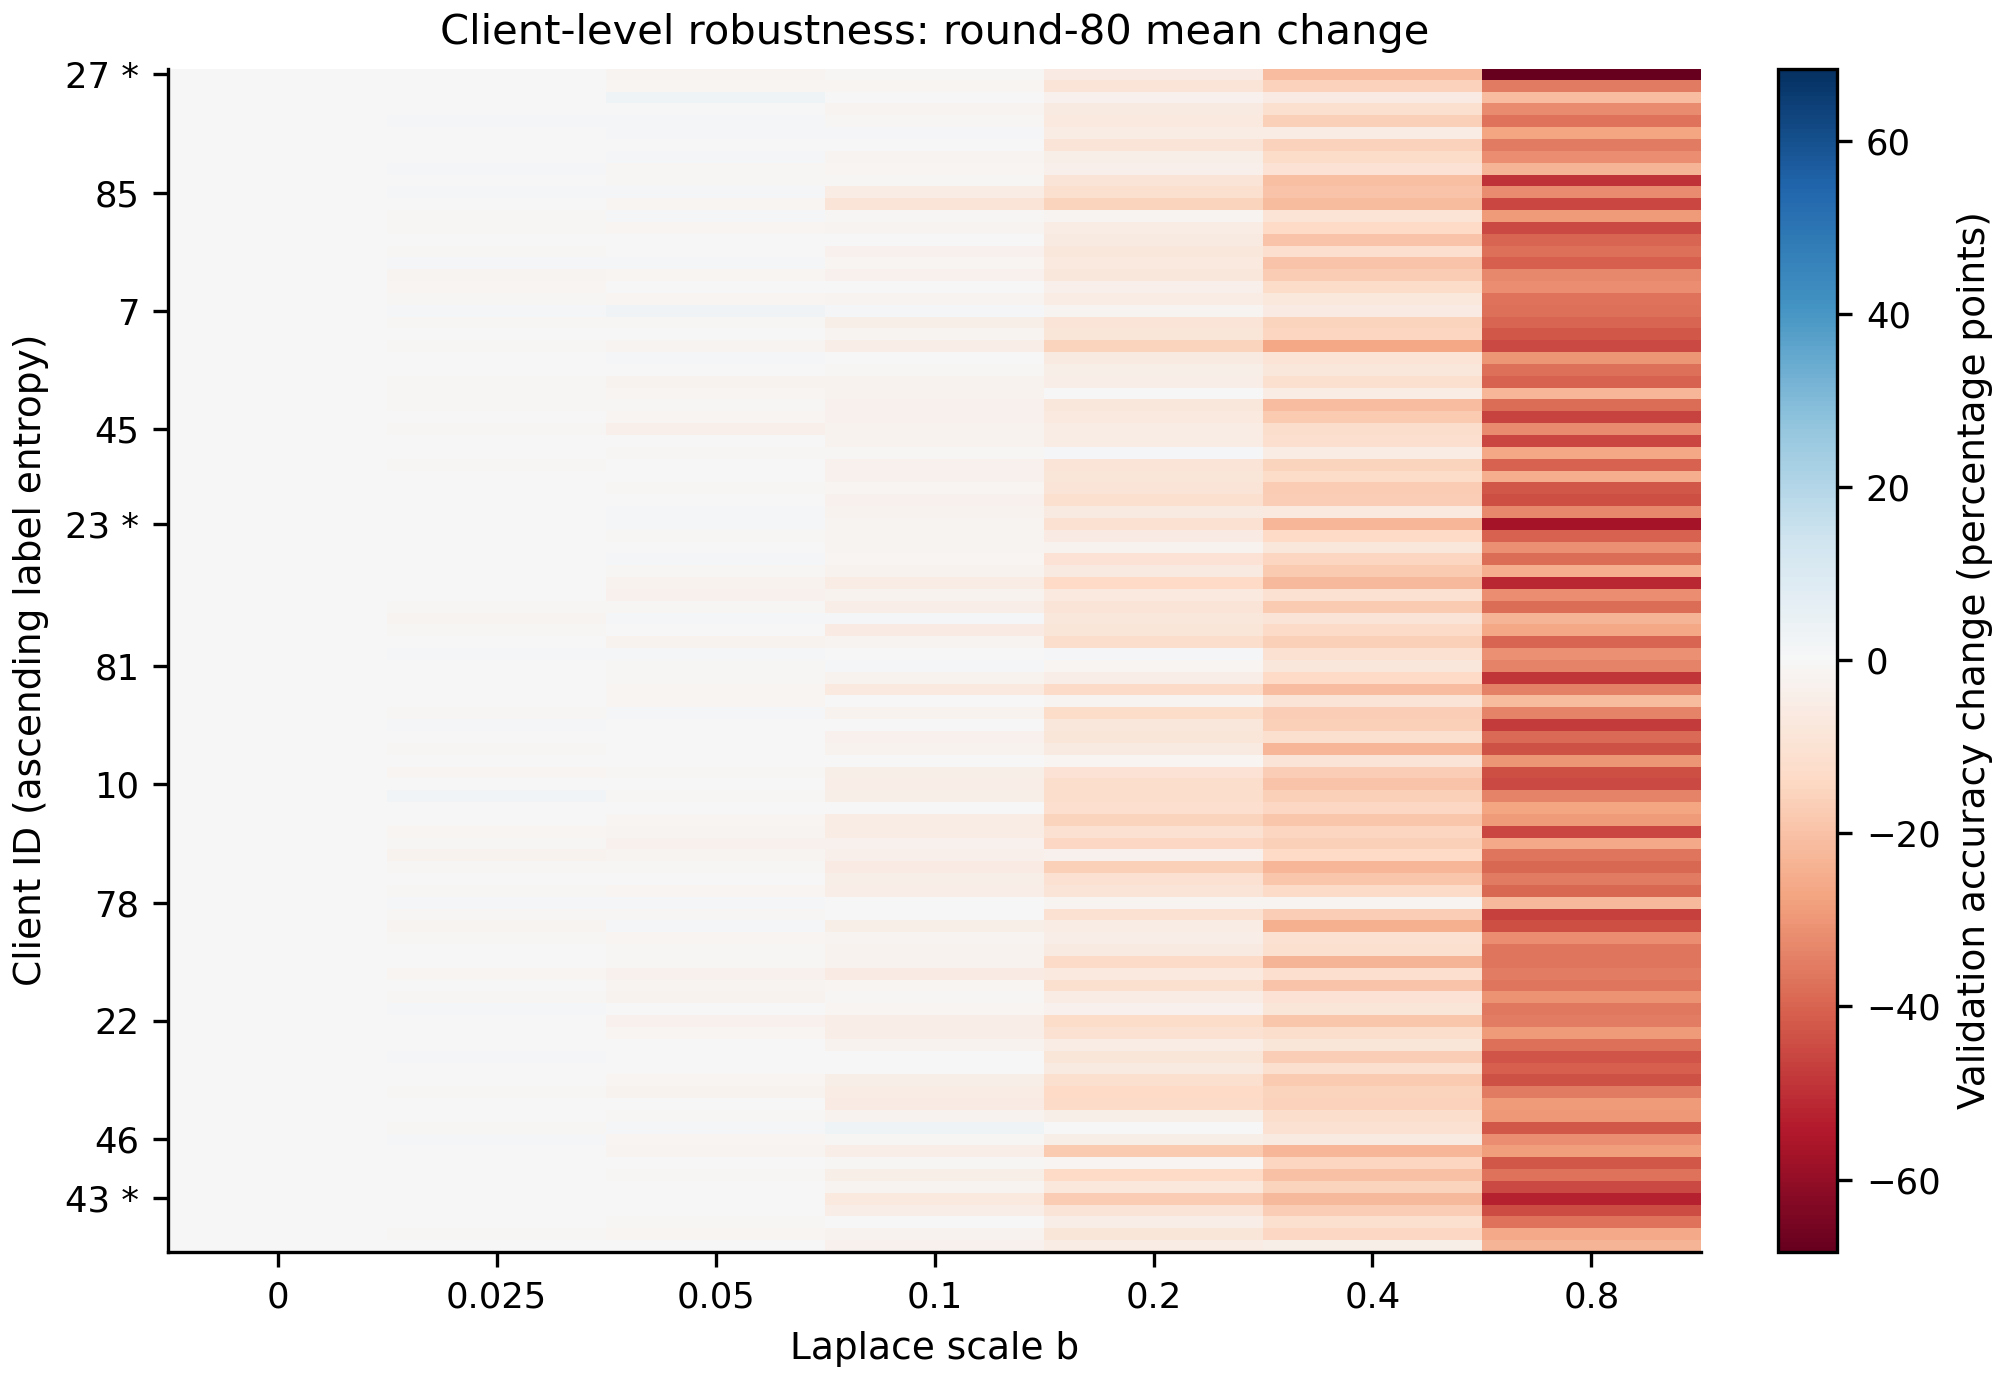
\includegraphics[width=\linewidth]{figures/part2/dp_client_robustness_heatmap.png}
\caption{Client-level changes in clean validation accuracy from matching $b=0$ controls, averaged over seeds 2026--2028 at round 80. Rows follow ascending training-label entropy. Stars mark clients 27, 23, and 43, the largest losses at $b=0.8$; the zero-noise column is identically zero.}\label{fig:robustness}
\end{figure}

Correlations of accuracy change with training size, entropy, and observed-class count are $-0.0385$, $-0.2305$, and $-0.2792$ at $b=0.10$, versus $-0.1743$, $0.0925$, and $-0.1477$ at $b=0.8$. Bottom/top size quartiles lose 34.60/39.22 points at $b=0.8$. The weak and changing associations describe heterogeneous sensitivity, without identifying a single causal predictor.

\subsubsection{Extreme noise, invalid inputs, and recovery}
Numerical stress tests distinguish finite deterioration from explicit failure. Client 25 trains for three local epochs at scales from $10^{-12}$ to $10^6$, with gradient and prediction monitoring and no clipping (\cref{tab:stress}). This is a local-update test, not a full federated trajectory.

\begin{table}[htbp]
\centering
\caption{Selected extreme-noise local stress outcomes on client 25. Finite confidence or loss does not imply valid classification.}\label{tab:stress}
\begin{tabularx}{\linewidth}{rYrr}
\toprule
$b$ & Outcome & Validation loss & Accuracy (\%)\\
\midrule
$10^{-12}$ & Finite; some float32 additions round away & 3.8003 & 4.17\\
1.6 & Finite & 3.9397 & 8.33\\
3.2 & Finite & 4.1622 & 0\\
10 & Finite; maximum $|\nabla|\approx1.07\times10^4$ & $1.19\times10^6$ & 0\\
100 & Finite; maximum $|\nabla|\approx1.12\times10^{13}$ & $9.03\times10^{22}$ & 0\\
1,000 & Explicit non-finite local-loss rejection & --- & ---\\
$10^6$ & Explicit non-finite local-loss rejection & --- & ---\\
\bottomrule
\end{tabularx}
\end{table}

At $b=10$, mean prediction confidence is 1.0 despite zero accuracy. At $b=1000$ and $10^6$, non-finite local loss is explicitly rejected and no failed update enters aggregation. Separate guards reject negative or non-finite scale, non-finite inputs, and float32 overflow.

A class-zero fixture with sizes $[0,1,2,7,101,23,3,9,11,13]$ tests empty/tiny clients, imbalance, missing classes, and interruption/resumption. Nine clients are eligible; resumed and uninterrupted parameters differ by 0.0. Client-specific keys regenerate the same fixed perturbations after restart.


\subsection{Privacy interpretation: what the experiment does and does not establish}\label{sec:privacy}
The course defines differential privacy through neighboring datasets and a bound on output-distribution changes \citep{courseDP}. For every neighboring pair $D\sim D'$ and measurable output set $A$, pure differential privacy requires
\begin{equation}
\Pr[M(D)\in A]\le e^{\varepsilon}\Pr[M(D')\in A].\label{eq:dp}
\end{equation}
For a query $f$ with specified sensitivity $\Delta_1f=\sup_{D\sim D'}\|f(D)-f(D')\|_1$, independent Laplace noise gives the classical calibration $\varepsilon=\Delta_1f/b$, or equivalently $b=\Delta_1f/\varepsilon$. Postprocessing preserves an already established guarantee, while multiple protected releases require an appropriate joint analysis or composition \citep{dworkroth2014}.

For an illustrative calibration, suppose the mechanism releases only one noisy normalized image, using independent, unpredictable private Laplace randomness, with no additional data-dependent outputs. Under \emph{pixel-level adjacency}, neighboring images differ in only one pixel by at most 1, so the identity query has $\Delta_1=1$ and $\varepsilon_{\mathrm{pixel}}=1/b$. At $b=0.05,0.10,0.20$, these values are 20, 10, and 5. Under \emph{whole-image replacement adjacency}, any image in $[0,1]^{784}$ may be replaced by another. The bound $\Delta_1\le784$ gives the worst-case calibration $\varepsilon_{\mathrm{image}}=784/b$: 15,680, 7,840, and 3,920 at the same scales, and 980 even at $b=0.80$. Thus the tested grid yields very loose worst-case whole-image guarantees for this hypothetical release; $b=0.05$ does not provide strong image-level privacy under this calibration.

These illustrative values are not privacy guarantees for the implemented FedAvg system. The experiment perturbs inputs rather than clipped gradients or model updates, and it implements no DP-SGD accountant. An end-to-end guarantee would require a protected unit (image or writer), adjacency relation, sensitivity bound, adversary model, and analysis of every released output.

Several outputs require protection beyond noisy images: labels, counts, and client IDs are unchanged; public reproducibility keys make noise reconstructible; and clean-data metrics access unperturbed examples. Multiple models, seeds, and metrics also enlarge the release surface. Fixed-noise reuse could invoke postprocessing only after establishing privacy for all information available to the learner and accounting for other releases. It does not automatically constitute a fresh release each epoch. Resampled noise requires a separate analysis.

Accordingly, $b=0.05$ remains the largest tested perturbation satisfying the predefined utility constraint. Its role is an empirical distortion--utility choice; deployment requiring verified image-level differential privacy would need a calibrated mechanism and complete accounting. No $\varepsilon$ is attributed to the actual trained FedAvg models or to the overall experimental pipeline.


